\begin{landscape}
\begin{figure}[p]\centering
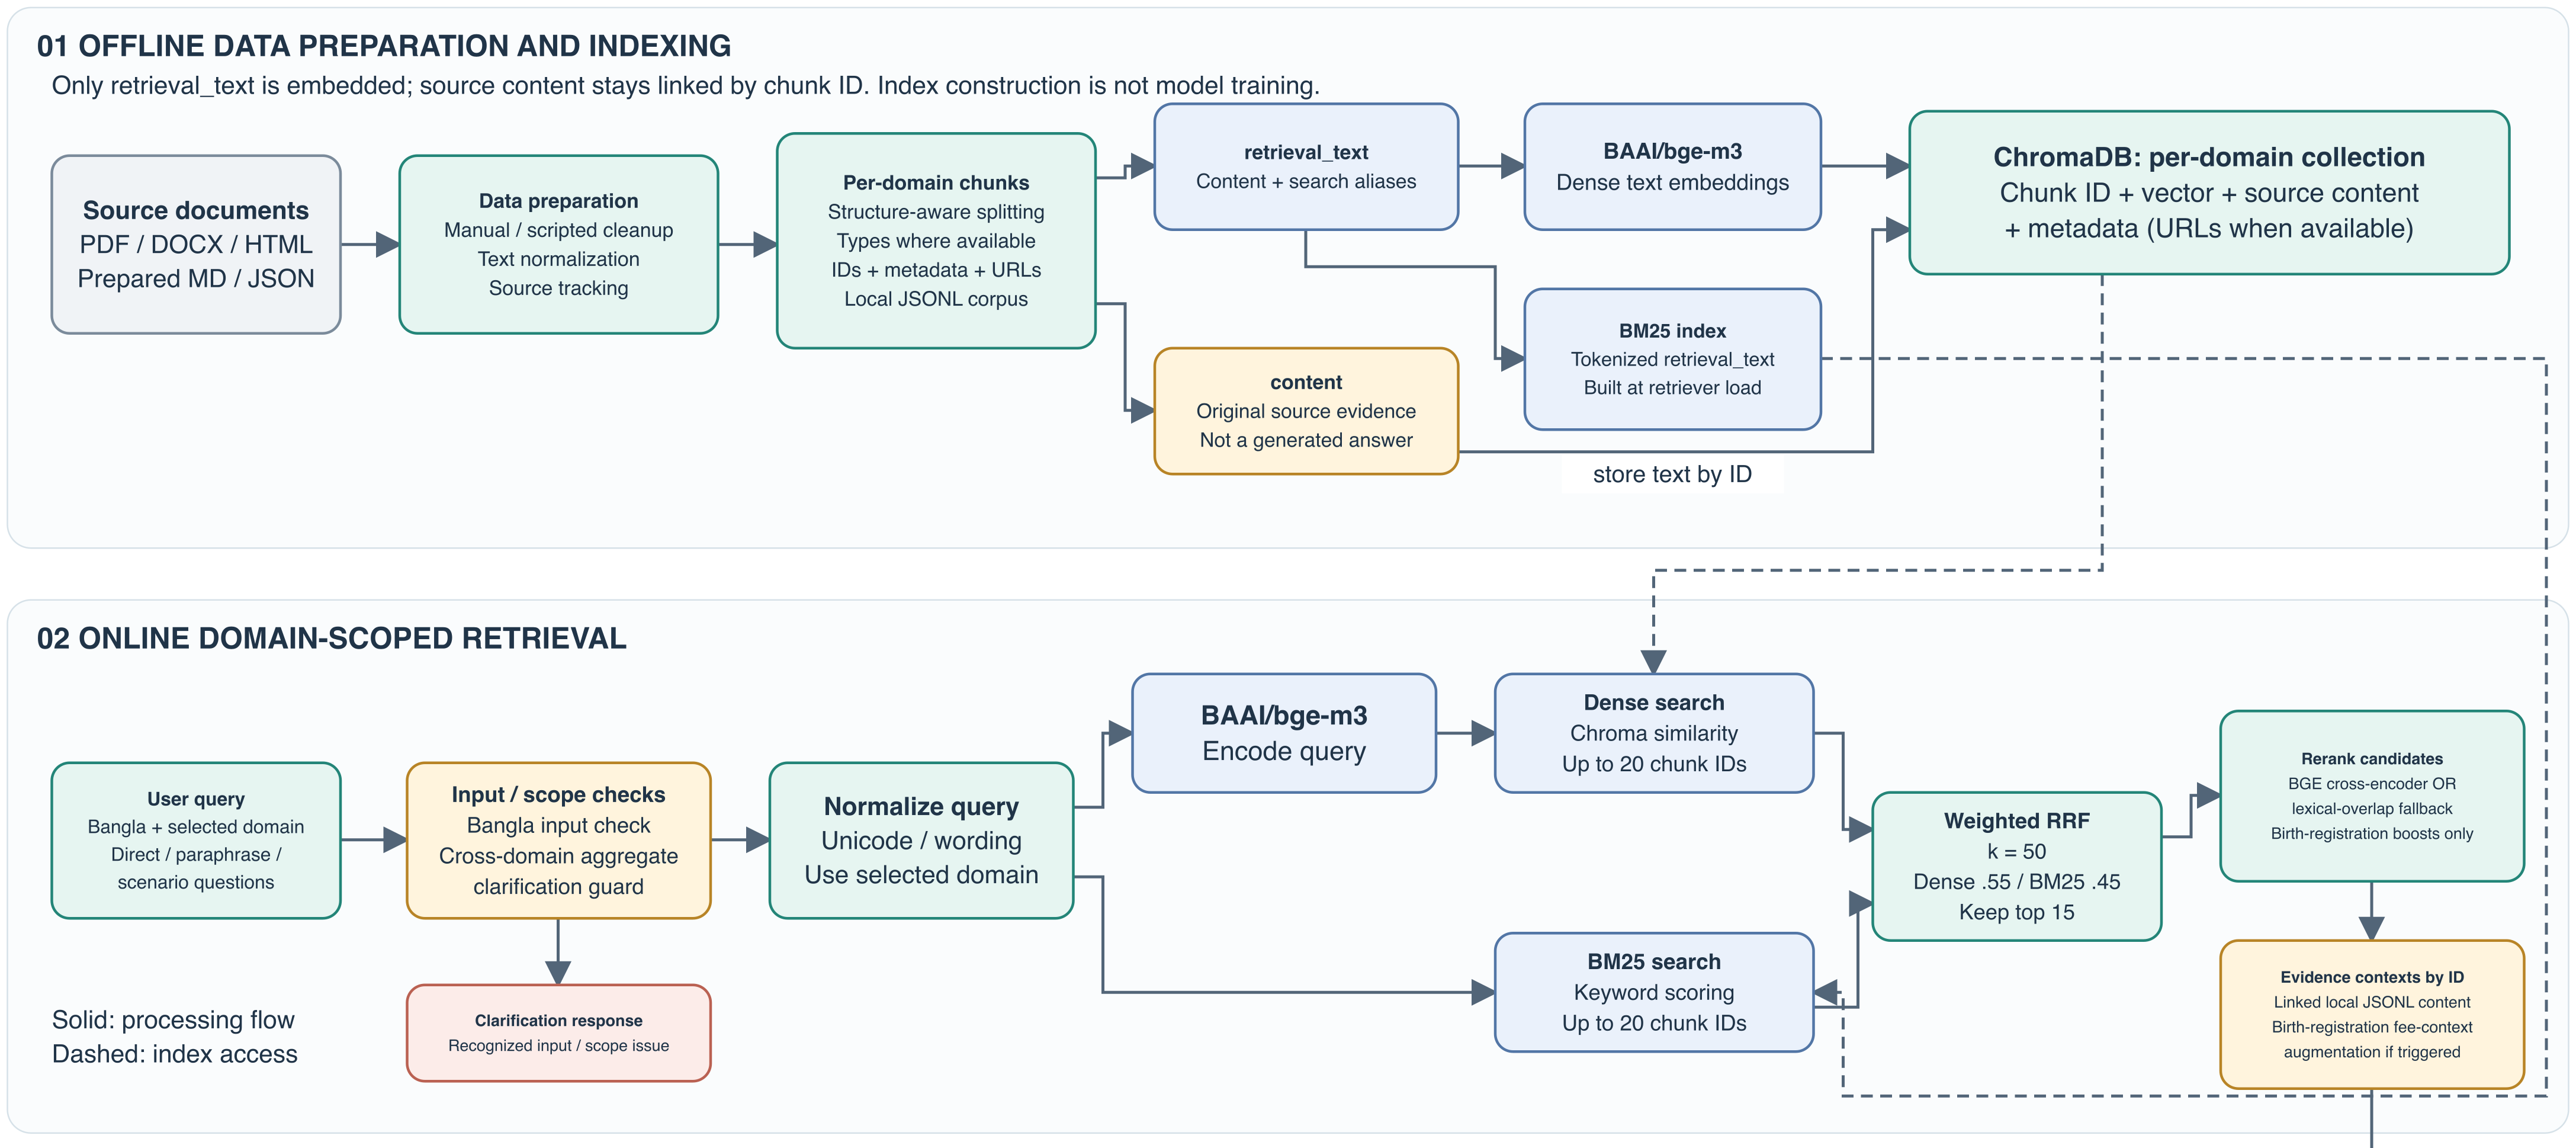
\includegraphics[width=\linewidth]{generated/architecture_retrieval.png}
\caption{CivicRAG offline preparation and online retrieval, exported from the editable architecture. Solid arrows show processing; dashed arrows indicate index access. The two retrieval channels share chunk identifiers, while additional registration-specific rules are conditional.}\label{fig:architecture}
\end{figure}
\end{landscape}
\begin{landscape}
\begin{figure}[p]\centering
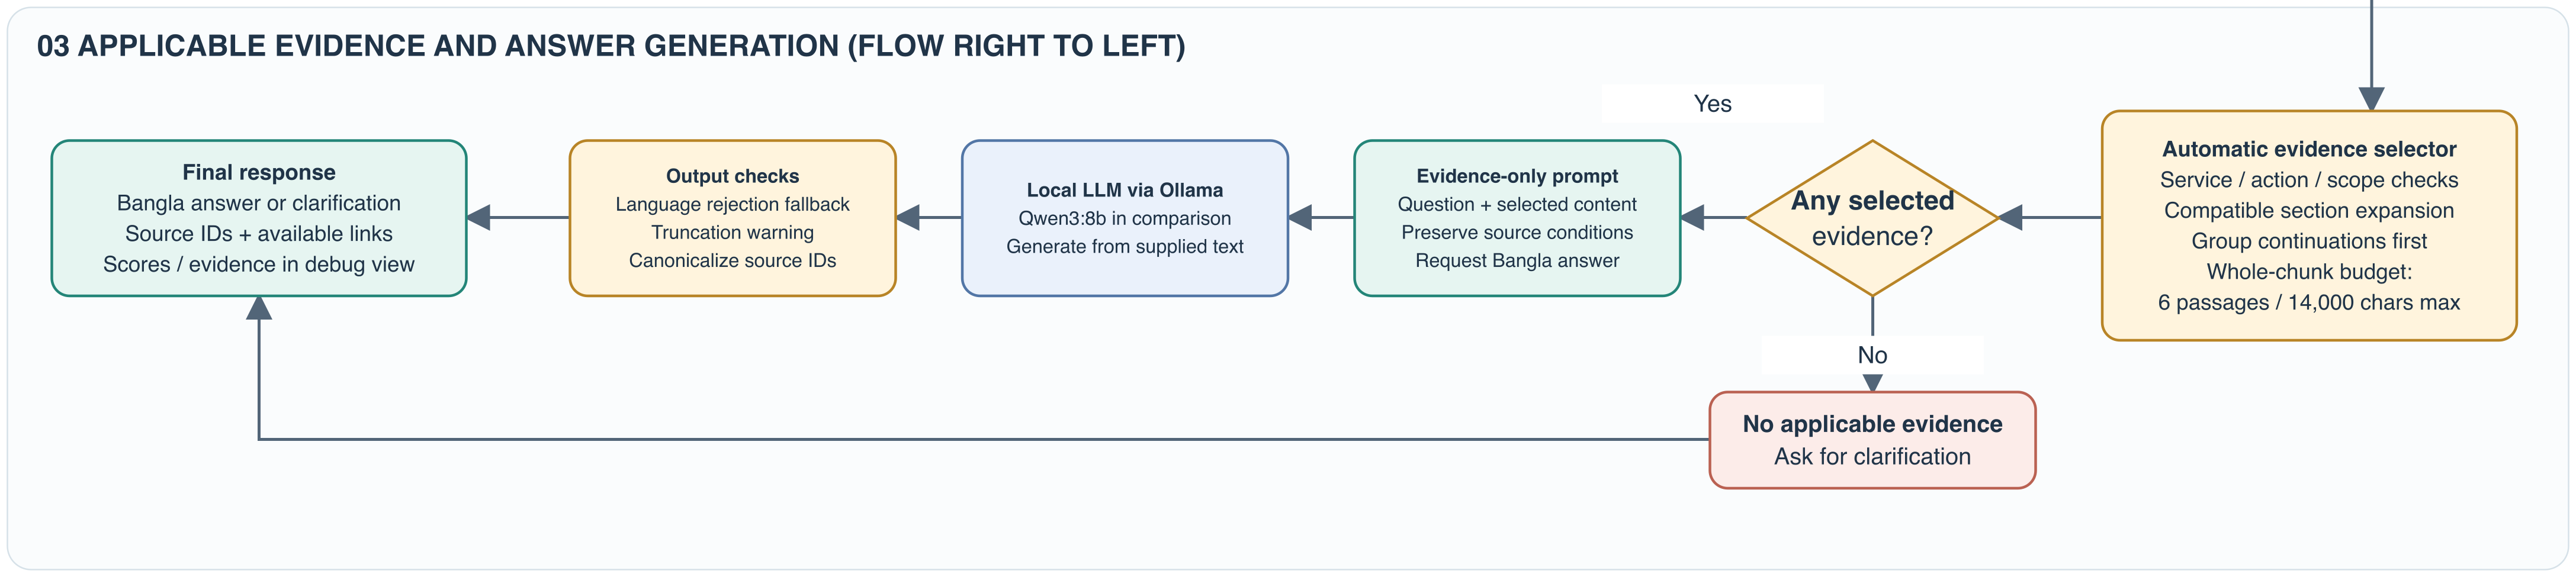
\includegraphics[width=\linewidth]{generated/architecture_generation.png}
\caption{CivicRAG evidence selection and generation, continuing from Figure~\ref{fig:architecture}. Flow is right to left. The selector is heuristic; an empty selection produces clarification. The output-check group includes operations in both the generator wrapper and pipeline. Source IDs identify supplied passages, not verified claim-level citations.}\label{fig:answer-architecture}
\end{figure}
\end{landscape}
\begin{landscape}
\begin{figure}[p]\centering
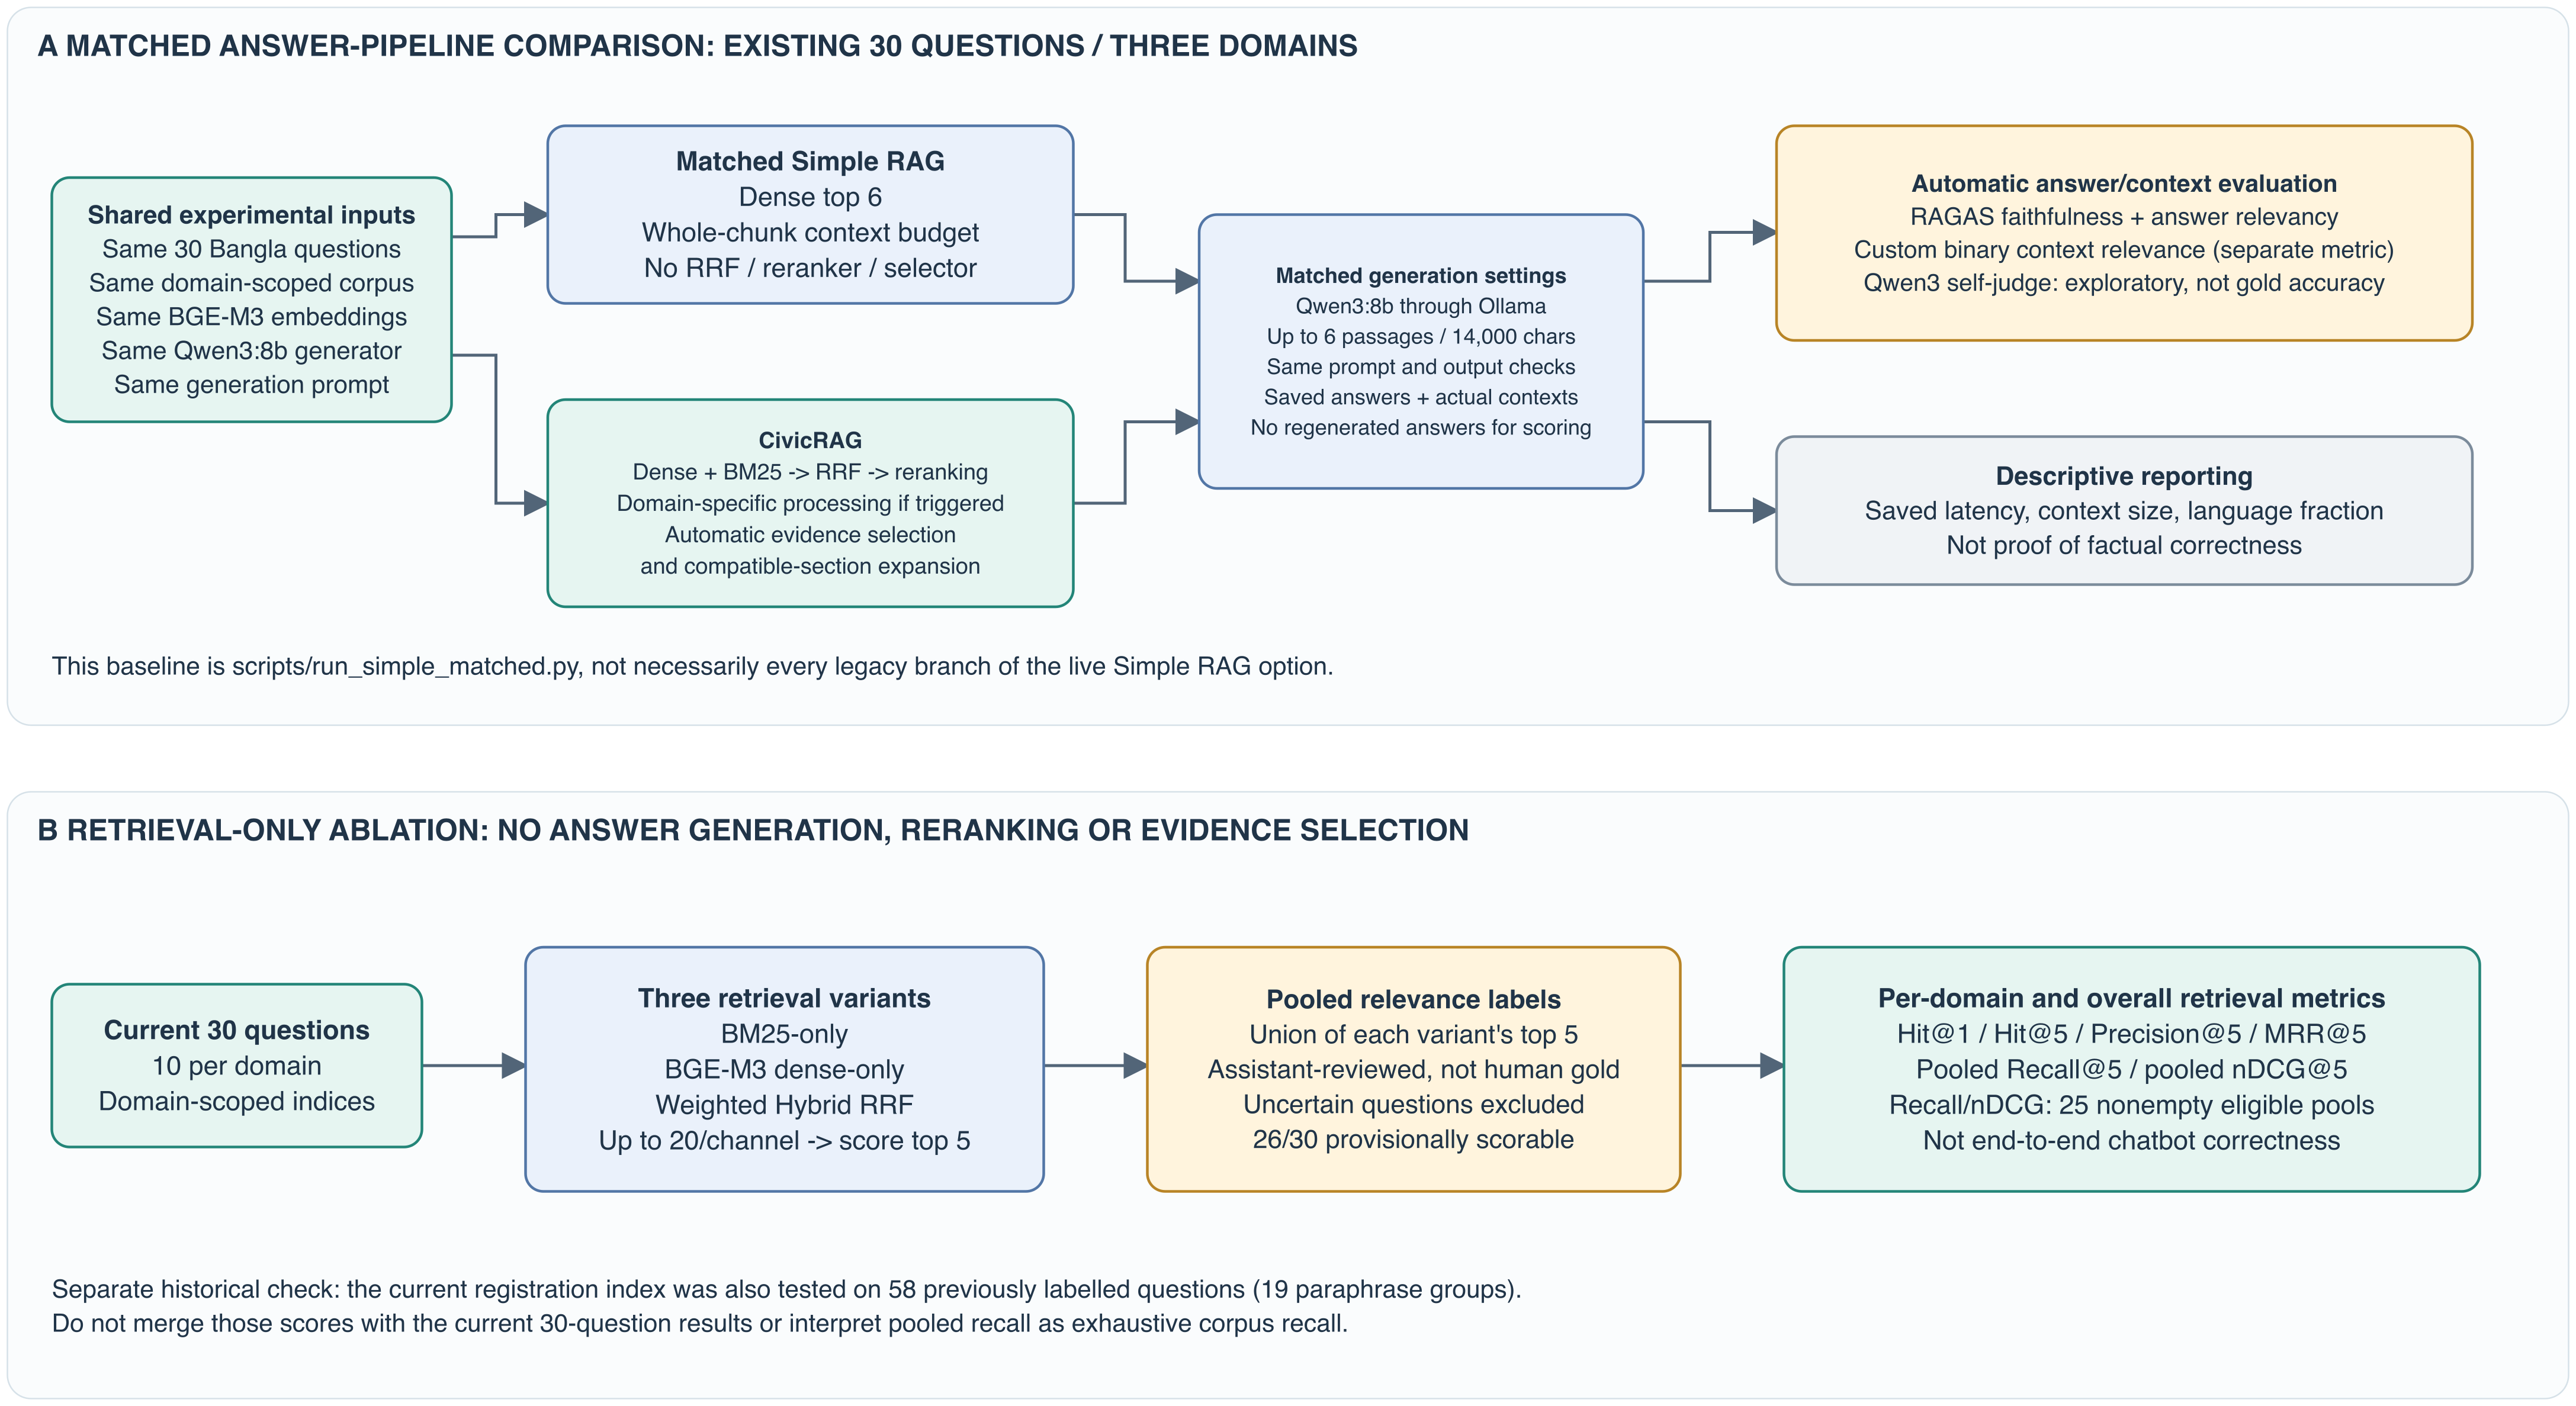
\includegraphics[width=\linewidth,height=0.84\textwidth,keepaspectratio]{generated/evaluation_design.png}
\caption{Evaluation boundaries. Panel A compares matched answer pipelines; Panel B evaluates retrieval before reranking and evidence selection. Assistant-reviewed pooled labels and local self-judge scores are explicitly separated from independent ground truth.}\label{fig:evaluation-architecture}
\end{figure}
\end{landscape}
